\begin{frame}
\frametitle{Va chạm}
Xét hai vật có khối lượng \(m_1\) và \(m_2\) chuyển động với vận tốc \(v_1\) và \(v_2\). Tìm vận tốc sau va chạm \(v_1'\) và \(v_2'\) của chúng. Biết rằng va chạm là hoàn toàn đàn hồi.
\begin{figure}
    \centering
    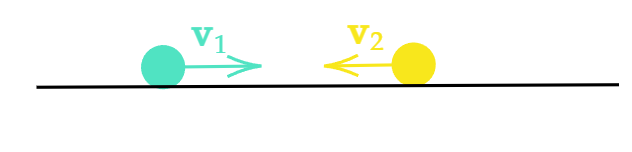
\includegraphics[width=0.4\textwidth]{Content/Figure/collision.png}
\end{figure}
\pause
\begin{columns}
\begin{column}{0.5\textwidth}
\scriptsize
Định luật bảo toàn động lượng:
\begin{equation*}
    m_1 v_1 - m_2 v_2 = m_1 v_1' - m_2 v_2'.
\end{equation*}
Định luật bảo toàn năng lượng:
\begin{equation*}
    \frac{m_1 v_1^2}{2} + \frac{m_2 v_2^2}{2} = \frac{m_1 {v_1'}^2}{2} + \frac{m_2 {v_2'}^2}{2}.
\end{equation*}
\normalsize
\end{column}
\begin{column}{0.5\textwidth}
Giải hệ phương trình trên ta được:
\begin{equation}
    \begin{aligned}
    v_1' = \frac{(m_1 - m_2)v_1 + 2m_2 v_2}{m_1 + m_2},\\
    v_2' = \frac{(m_2 - m_1)v_2 + 2m_1 v_1}{m_1 + m_2}.
    \end{aligned}
\end{equation}
\end{column}
\end{columns}
\end{frame}

\begin{frame}
\frametitle{Dao động nhỏ}
Xét một vật có khối lượng \(m\) chuyển động trong thế năng \(U(q)\) với vị trí cân bằng tại \(q_0\) (tức là \(U'(q_0)=0\)). Nếu vật bị lệch một khoảng rất nhỏ \(\eta=q-q_0\), vật sẽ dao động gần như điều hòa. Tìm tần số góc của dao động này.
\begin{columns}
\begin{column}{0.5\textwidth}
\begin{figure}
    \centering
    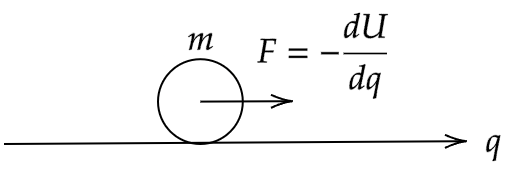
\includegraphics[width=0.8\textwidth]{Content/Figure/small oscillation.png}
\end{figure}
\end{column}
\begin{column}{0.5\textwidth}
\begin{figure}
    \centering
    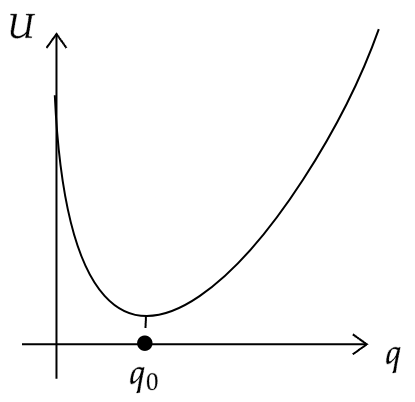
\includegraphics[width=0.5\textwidth]{Content/Figure/DaoDongNho.png}
\end{figure}
\end{column}
\end{columns}
\end{frame}

\begin{frame}
    \frametitle{Dao động nhỏ}   
    Khai triển Taylor thế năng quanh vị trí cân bằng:
    \begin{equation*}
        U(q)=U(q_0)+U'(q_0)+\frac{U''(q_0)}{2}(q-q_0)^2+\ldots
    \end{equation*}
    Số hạng đầu tiên là hằng số, có thể triệt tiêu tùy vào cách ta chọn mốc thế năng. Số hạng thứ hai bằng 0 do \(q_0\) là vị trí cân bằng. Do đó, ta chỉ quan tâm đến số hạng bậc 2 của \(U\):
    \begin{equation*}
        U(q)\approx \frac{U''(q_0)}{2}(q-q_0)^2.
    \end{equation*}
    Số hạng này có dạng giống như thế năng của lò xo, với độ cứng \(k=U''(q_0)\). Tần số góc của dao động nhỏ là:
    \begin{equation}
        \omega=\sqrt{\frac{U''(q_0)}{m}}.
    \end{equation}
\end{frame}

\begin{frame}
\frametitle{Lực xuyên tâm}
Một vật khối lượng \(m\) chuyển động trong một trường thế \(U(r)=-\dfrac{\alpha}{r}\) với \(r\) là khoảng cách từ vật đến một điểm cố định \(O\). Biết rằng tại một thời điểm nào đó, vật đang có mô men động lượng quanh \(O\) là \(L\), cơ năng \(E\) (\(E<0\)). Tìm bán kính nhỏ nhất và lớn nhất trong quỹ đạo của vật.
\begin{figure}
    \centering
    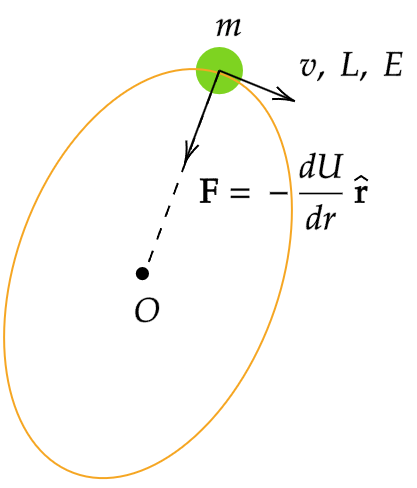
\includegraphics[width=0.25\textwidth]{Content/Figure/lucxuyentam.png}
\end{figure}
\end{frame}

\begin{frame}
\frametitle{Lực xuyên tâm}
\scriptsize
Tại điểm cực cận và cực viễn của quỹ đạo, vận tốc của vật vuông góc với \(\mathbf r\).

Định luật bảo toàn mô men động lượng quanh O:
\begin{equation*}
    m v r= const = L.
\end{equation*}
Định luật bảo toàn cơ năng:
\begin{equation*}
    \frac{m v^2}{2} - \dfrac{\alpha}{r} = const = E.
\end{equation*}
Giải hệ phương trình trên, ta thu được phương trình bậc 2 của \(r\):
\begin{equation*}
    -E r^2 - \alpha r + \frac{L^2}{2m} = 0.
\end{equation*}
Từ đó, ta tìm được bán kính cực cận và cực viễn:
\begin{equation}
    r_{min,max} = \frac{\alpha \pm \sqrt{\alpha^2 + 2 E L^2 / m}}{-2E}.
\end{equation}
\normalsize
\end{frame}